%!TEX encoding = UTF-8 Unicode

\documentclass[landscape]{book}
\usepackage[a3paper]{geometry}

\usepackage{verbatim}

\usepackage{hyperref}

\usepackage{tikz}

\usetikzlibrary{
  arrows,
  shapes.misc,% wg. rounded rectangle
  shapes.arrows,%
  matrix,%
  scopes,%
  shadows%
}

\tikzset{
  nonterminal/.style={
    % The shape:
    rectangle,
    % The size:
    minimum size=6mm,
    % The border:
    very thick,
    draw=red!50!black!50,         % 50% red and 50% black,
                                  % and that mixed with 50% white
    % The filling:
    top color=white,              % a shading that is white at the top...
    bottom color=red!50!black!20, % and something else at the bottom
    % Font
    font=\itshape\small
  },
  terminal/.style={
    % The shape:
    rounded rectangle,
    minimum size=6mm,
    % The rest
    very thick,draw=black!50,
    top color=white,bottom color=black!20,
    font=\ttfamily\small
  },
  firstPoint/.style={circle,>=stealth',thick,draw=black!50},
  point/.style={coordinate,>=stealth',thick,draw=black!50},
  tip/.style={->,shorten >=0.007pt},
  lastPoint/.style={rectangle,>=stealth',thick,draw=black!50},
  every join/.style={rounded corners}
}

\newcommand\nonTerminalSection[2]{\section{Nonterminal \texttt{#1}}\label{nt:#2}}
\newcommand\ruleSubsection[3]{\subsection{Component \texttt{#1}, in file \texttt{#2}, line #3}}
\newcommand\ruleMatrixColumnSeparation{3mm}
\newcommand\ruleMatrixRowSeparation{3mm}
\newcommand\nonTerminalSymbol[2]{\hyperref[nt:#2]{#1}}
\newcommand\startSymbol[2]{The start symbol is \hyperref[nt:#2]{#1}.}

\newcommand\nonTerminalSummaryStart{This is the alphabetical list of non terminal : }
\newcommand\nonTerminalSummary[2]{\hyperref[nt:#2]{#1}}
\newcommand\nonTerminalSummarySeparator{, }
\newcommand\nonTerminalSummaryEnd{.\\}

\begin{document}

\title{\Huge{Grammar \texttt{goil\_object\_level\_include}}}
\date \today 

\maketitle

\startSymbol{oil\_declaration\_list}{9}

\nonTerminalSummaryStart \nonTerminalSummary{OIL\_version}{5}\nonTerminalSummarySeparator \nonTerminalSummary{application\_definition}{6}\nonTerminalSummarySeparator \nonTerminalSummary{boolean}{8}\nonTerminalSummarySeparator \nonTerminalSummary{description}{4}\nonTerminalSummarySeparator \nonTerminalSummary{file}{2}\nonTerminalSummarySeparator \nonTerminalSummary{implementation\_definition}{0}\nonTerminalSummarySeparator \nonTerminalSummary{include\_cpu\_level}{12}\nonTerminalSummarySeparator \nonTerminalSummary{include\_file\_level}{11}\nonTerminalSummarySeparator \nonTerminalSummary{include\_object\_level}{13}\nonTerminalSummarySeparator \nonTerminalSummary{object\_definition\_list}{7}\nonTerminalSummarySeparator \nonTerminalSummary{oil\_declaration}{10}\nonTerminalSummarySeparator \nonTerminalSummary{oil\_declaration\_list}{9}\nonTerminalSummarySeparator \nonTerminalSummary{sign}{3}\nonTerminalSummarySeparator \nonTerminalSummary{start}{1}\nonTerminalSummaryEnd \nonTerminalSection{OIL\_version}{5}

\ruleSubsection{goil\_syntax}{goil\_syntax}{163}

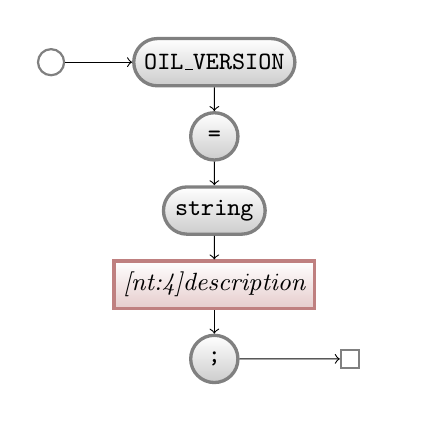
\begin{tikzpicture}
  \matrix[column sep=\ruleMatrixColumnSeparation, row sep=\ruleMatrixRowSeparation] {
    \node (P0start) [firstPoint] {}; & & \node (p4-2) [terminal] {OIL\_VERSION}; & \\
    & & \node (p3-2) [terminal] {=}; & \\
    & & \node (p2-2) [terminal] {string}; & \\
    & & \node (p1-2) [nonterminal] {\nonTerminalSymbol{description}{4}}; & \\
    & & \node (p0-2) [terminal] {;}; & \node (p0-3) [lastPoint] {}; & \\
  };
  \draw[->] (P0start) -- (p4-2) ;
  \draw[->] (p4-2) -- (p3-2) ;
  \draw[->] (p3-2) -- (p2-2) ;
  \draw[->] (p2-2) -- (p1-2) ;
  \draw[->] (p1-2) -- (p0-2) ;
  \draw[->] (p0-2) -- (p0-3) ;
\end{tikzpicture}

\nonTerminalSection{application\_definition}{6}

\ruleSubsection{goil\_syntax}{goil\_syntax}{170}

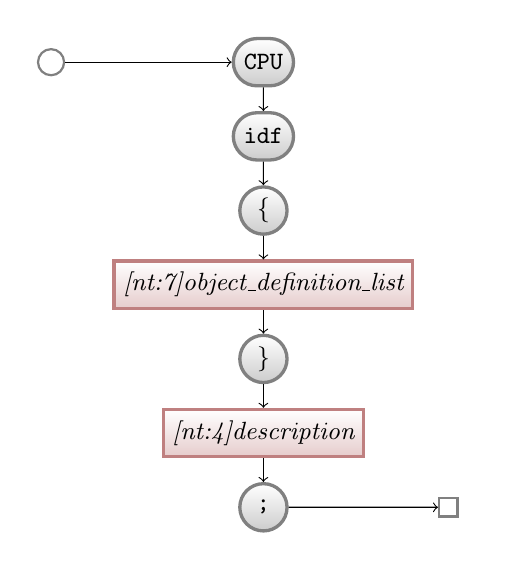
\begin{tikzpicture}
  \matrix[column sep=\ruleMatrixColumnSeparation, row sep=\ruleMatrixRowSeparation] {
    \node (P0start) [firstPoint] {}; & & \node (p6-2) [terminal] {CPU}; & \\
    & & \node (p5-2) [terminal] {idf}; & \\
    & & \node (p4-2) [terminal] {\{}; & \\
    & & \node (p3-2) [nonterminal] {\nonTerminalSymbol{object\_definition\_list}{7}}; & \\
    & & \node (p2-2) [terminal] {\}}; & \\
    & & \node (p1-2) [nonterminal] {\nonTerminalSymbol{description}{4}}; & \\
    & & \node (p0-2) [terminal] {;}; & \node (p0-3) [lastPoint] {}; & \\
  };
  \draw[->] (P0start) -- (p6-2) ;
  \draw[->] (p6-2) -- (p5-2) ;
  \draw[->] (p5-2) -- (p4-2) ;
  \draw[->] (p4-2) -- (p3-2) ;
  \draw[->] (p3-2) -- (p2-2) ;
  \draw[->] (p2-2) -- (p1-2) ;
  \draw[->] (p1-2) -- (p0-2) ;
  \draw[->] (p0-2) -- (p0-3) ;
\end{tikzpicture}

\nonTerminalSection{boolean}{8}

\ruleSubsection{goil\_syntax}{goil\_syntax}{234}

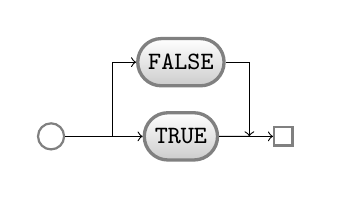
\begin{tikzpicture}
  \matrix[column sep=\ruleMatrixColumnSeparation, row sep=\ruleMatrixRowSeparation] {
    & & & \node (p1-3) [terminal] {FALSE}; & \\
    \node (P0start) [firstPoint] {}; & & \node (p0-2) [point] {}; & \node (p0-3) [terminal] {TRUE}; & \node (p0-4) [point] {}; & \node (p0-5) [lastPoint] {}; & \\
  };
  \draw[->] (P0start) -- (p0-3) ;
  \draw[->] (p0-2) |- (p1-3) ;
  \draw (p0-3) -- (p0-4) ;
  \draw[->] (p1-3) -| (p0-4) ;
  \draw[->] (p0-4) -- (p0-5) ;
\end{tikzpicture}

\nonTerminalSection{description}{4}

\ruleSubsection{goil\_syntax}{goil\_syntax}{139}

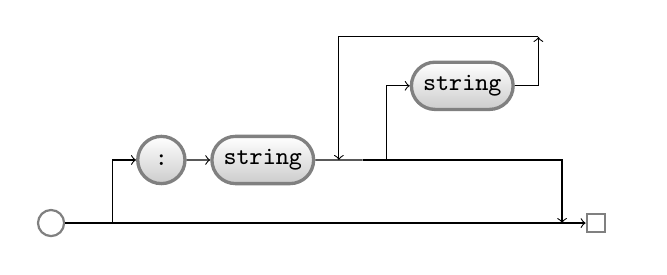
\begin{tikzpicture}
  \matrix[column sep=\ruleMatrixColumnSeparation, row sep=\ruleMatrixRowSeparation] {
    & & & & & & & & & \node (p3-9) [point] {}; & \\
    & & & & & & & & \node (p2-8) [terminal] {string}; & \\
    & & & \node (p1-3) [terminal] {:}; & \node (p1-4) [terminal] {string}; & \node (p1-5) [point] {}; & \node (p1-6) [point] {}; & \node (p1-7) [point] {}; & \\
    \node (P0start) [firstPoint] {}; & & \node (p0-2) [point] {}; & \node (p0-3) [point] {}; & & & & & & & \node (p0-10) [point] {}; & \node (p0-11) [lastPoint] {}; & \\
  };
  \draw (P0start) -- (p0-3) ;
  \draw[->] (p0-2) |- (p1-3) ;
  \draw[->] (p1-3) -- (p1-4) ;
  \draw (p1-4) -- (p1-6) ;
  \draw[->] (p1-7) |- (p2-8) ;
  \draw[->] (p3-9) -| (p1-5) ;
  \draw[->] (p2-8) -| (p3-9) ;
  \draw (p0-3) -- (p0-10) ;
  \draw[->] (p1-6) -| (p0-10) ;
  \draw[->] (p0-10) -- (p0-11) ;
\end{tikzpicture}

\nonTerminalSection{file}{2}

\ruleSubsection{goil\_syntax}{goil\_syntax}{110}

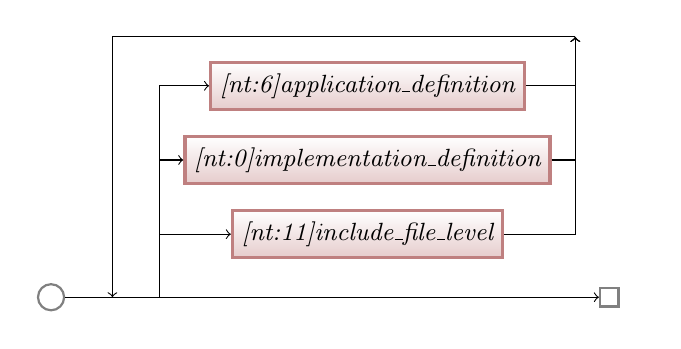
\begin{tikzpicture}
  \matrix[column sep=\ruleMatrixColumnSeparation, row sep=\ruleMatrixRowSeparation] {
    & & & & & & \node (p4-6) [point] {}; & \\
    & & & & & \node (p3-5) [nonterminal] {\nonTerminalSymbol{application\_definition}{6}}; & \\
    & & & & & \node (p2-5) [nonterminal] {\nonTerminalSymbol{implementation\_definition}{0}}; & \\
    & & & & & \node (p1-5) [nonterminal] {\nonTerminalSymbol{include\_file\_level}{11}}; & \\
    \node (P0start) [firstPoint] {}; & & \node (p0-2) [point] {}; & \node (p0-3) [point] {}; & \node (p0-4) [point] {}; & & & \node (p0-7) [lastPoint] {}; & \\
  };
  \draw (P0start) -- (p0-3) ;
  \draw[->] (p0-4) |- (p1-5) ;
  \draw[->] (p0-4) |- (p2-5) ;
  \draw[->] (p0-4) |- (p3-5) ;
  \draw[->] (p4-6) -| (p0-2) ;
  \draw[->] (p1-5) -| (p4-6) ;
  \draw[->] (p2-5) -| (p4-6) ;
  \draw[->] (p3-5) -| (p4-6) ;
  \draw[->] (p0-3) -- (p0-7) ;
\end{tikzpicture}

\nonTerminalSection{implementation\_definition}{0}

\nonTerminalSection{include\_cpu\_level}{12}

\ruleSubsection{goil\_syntax}{goil\_syntax}{475}

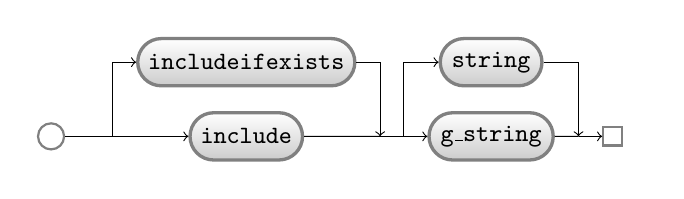
\begin{tikzpicture}
  \matrix[column sep=\ruleMatrixColumnSeparation, row sep=\ruleMatrixRowSeparation] {
    & & & \node (p1-3) [terminal] {includeifexists}; & & & \node (p1-6) [terminal] {string}; & \\
    \node (P0start) [firstPoint] {}; & & \node (p0-2) [point] {}; & \node (p0-3) [terminal] {include}; & \node (p0-4) [point] {}; & \node (p0-5) [point] {}; & \node (p0-6) [terminal] {g\_string}; & \node (p0-7) [point] {}; & \node (p0-8) [lastPoint] {}; & \\
  };
  \draw[->] (P0start) -- (p0-3) ;
  \draw[->] (p0-2) |- (p1-3) ;
  \draw (p0-3) -- (p0-4) ;
  \draw[->] (p1-3) -| (p0-4) ;
  \draw[->] (p0-4) -- (p0-6) ;
  \draw[->] (p0-5) |- (p1-6) ;
  \draw (p0-6) -- (p0-7) ;
  \draw[->] (p1-6) -| (p0-7) ;
  \draw[->] (p0-7) -- (p0-8) ;
\end{tikzpicture}

\nonTerminalSection{include\_file\_level}{11}

\ruleSubsection{goil\_syntax}{goil\_syntax}{451}

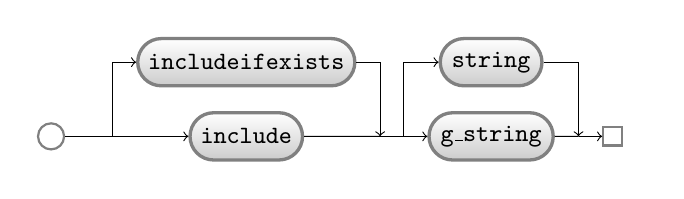
\begin{tikzpicture}
  \matrix[column sep=\ruleMatrixColumnSeparation, row sep=\ruleMatrixRowSeparation] {
    & & & \node (p1-3) [terminal] {includeifexists}; & & & \node (p1-6) [terminal] {string}; & \\
    \node (P0start) [firstPoint] {}; & & \node (p0-2) [point] {}; & \node (p0-3) [terminal] {include}; & \node (p0-4) [point] {}; & \node (p0-5) [point] {}; & \node (p0-6) [terminal] {g\_string}; & \node (p0-7) [point] {}; & \node (p0-8) [lastPoint] {}; & \\
  };
  \draw[->] (P0start) -- (p0-3) ;
  \draw[->] (p0-2) |- (p1-3) ;
  \draw (p0-3) -- (p0-4) ;
  \draw[->] (p1-3) -| (p0-4) ;
  \draw[->] (p0-4) -- (p0-6) ;
  \draw[->] (p0-5) |- (p1-6) ;
  \draw (p0-6) -- (p0-7) ;
  \draw[->] (p1-6) -| (p0-7) ;
  \draw[->] (p0-7) -- (p0-8) ;
\end{tikzpicture}

\nonTerminalSection{include\_object\_level}{13}

\ruleSubsection{goil\_syntax}{goil\_syntax}{499}

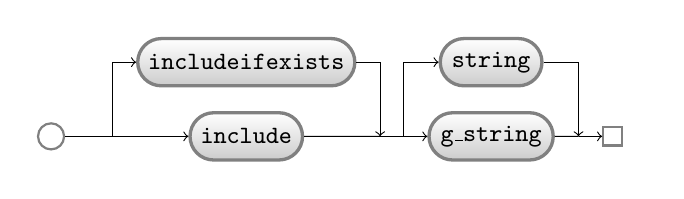
\begin{tikzpicture}
  \matrix[column sep=\ruleMatrixColumnSeparation, row sep=\ruleMatrixRowSeparation] {
    & & & \node (p1-3) [terminal] {includeifexists}; & & & \node (p1-6) [terminal] {string}; & \\
    \node (P0start) [firstPoint] {}; & & \node (p0-2) [point] {}; & \node (p0-3) [terminal] {include}; & \node (p0-4) [point] {}; & \node (p0-5) [point] {}; & \node (p0-6) [terminal] {g\_string}; & \node (p0-7) [point] {}; & \node (p0-8) [lastPoint] {}; & \\
  };
  \draw[->] (P0start) -- (p0-3) ;
  \draw[->] (p0-2) |- (p1-3) ;
  \draw (p0-3) -- (p0-4) ;
  \draw[->] (p1-3) -| (p0-4) ;
  \draw[->] (p0-4) -- (p0-6) ;
  \draw[->] (p0-5) |- (p1-6) ;
  \draw (p0-6) -- (p0-7) ;
  \draw[->] (p1-6) -| (p0-7) ;
  \draw[->] (p0-7) -- (p0-8) ;
\end{tikzpicture}

\nonTerminalSection{object\_definition\_list}{7}

\ruleSubsection{goil\_syntax}{goil\_syntax}{184}

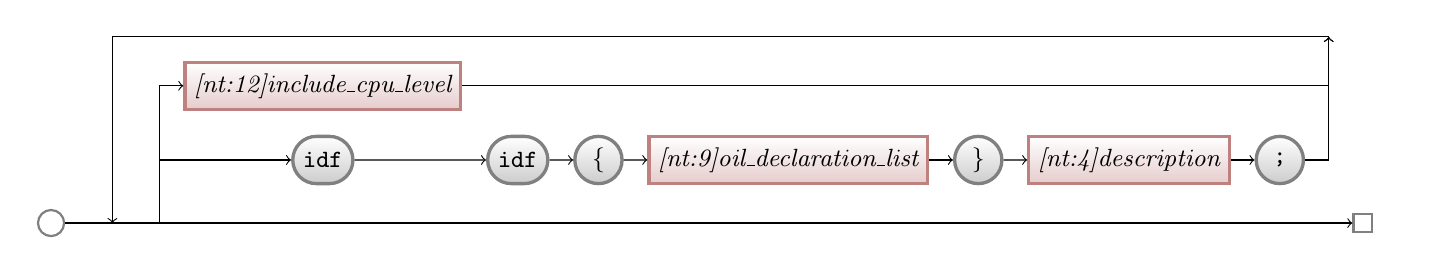
\begin{tikzpicture}
  \matrix[column sep=\ruleMatrixColumnSeparation, row sep=\ruleMatrixRowSeparation] {
    & & & & & & & & & & & & \node (p3-12) [point] {}; & \\
    & & & & & \node (p2-5) [nonterminal] {\nonTerminalSymbol{include\_cpu\_level}{12}}; & \\
    & & & & & \node (p1-5) [terminal] {idf}; & \node (p1-6) [terminal] {idf}; & \node (p1-7) [terminal] {\{}; & \node (p1-8) [nonterminal] {\nonTerminalSymbol{oil\_declaration\_list}{9}}; & \node (p1-9) [terminal] {\}}; & \node (p1-10) [nonterminal] {\nonTerminalSymbol{description}{4}}; & \node (p1-11) [terminal] {;}; & \\
    \node (P0start) [firstPoint] {}; & & \node (p0-2) [point] {}; & \node (p0-3) [point] {}; & \node (p0-4) [point] {}; & & & & & & & & & \node (p0-13) [lastPoint] {}; & \\
  };
  \draw (P0start) -- (p0-3) ;
  \draw[->] (p0-4) |- (p1-5) ;
  \draw[->] (p1-5) -- (p1-6) ;
  \draw[->] (p1-6) -- (p1-7) ;
  \draw[->] (p1-7) -- (p1-8) ;
  \draw[->] (p1-8) -- (p1-9) ;
  \draw[->] (p1-9) -- (p1-10) ;
  \draw[->] (p1-10) -- (p1-11) ;
  \draw[->] (p0-4) |- (p2-5) ;
  \draw[->] (p3-12) -| (p0-2) ;
  \draw[->] (p1-11) -| (p3-12) ;
  \draw[->] (p2-5) -| (p3-12) ;
  \draw[->] (p0-3) -- (p0-13) ;
\end{tikzpicture}

\nonTerminalSection{oil\_declaration}{10}

\ruleSubsection{goil\_syntax}{goil\_syntax}{256}

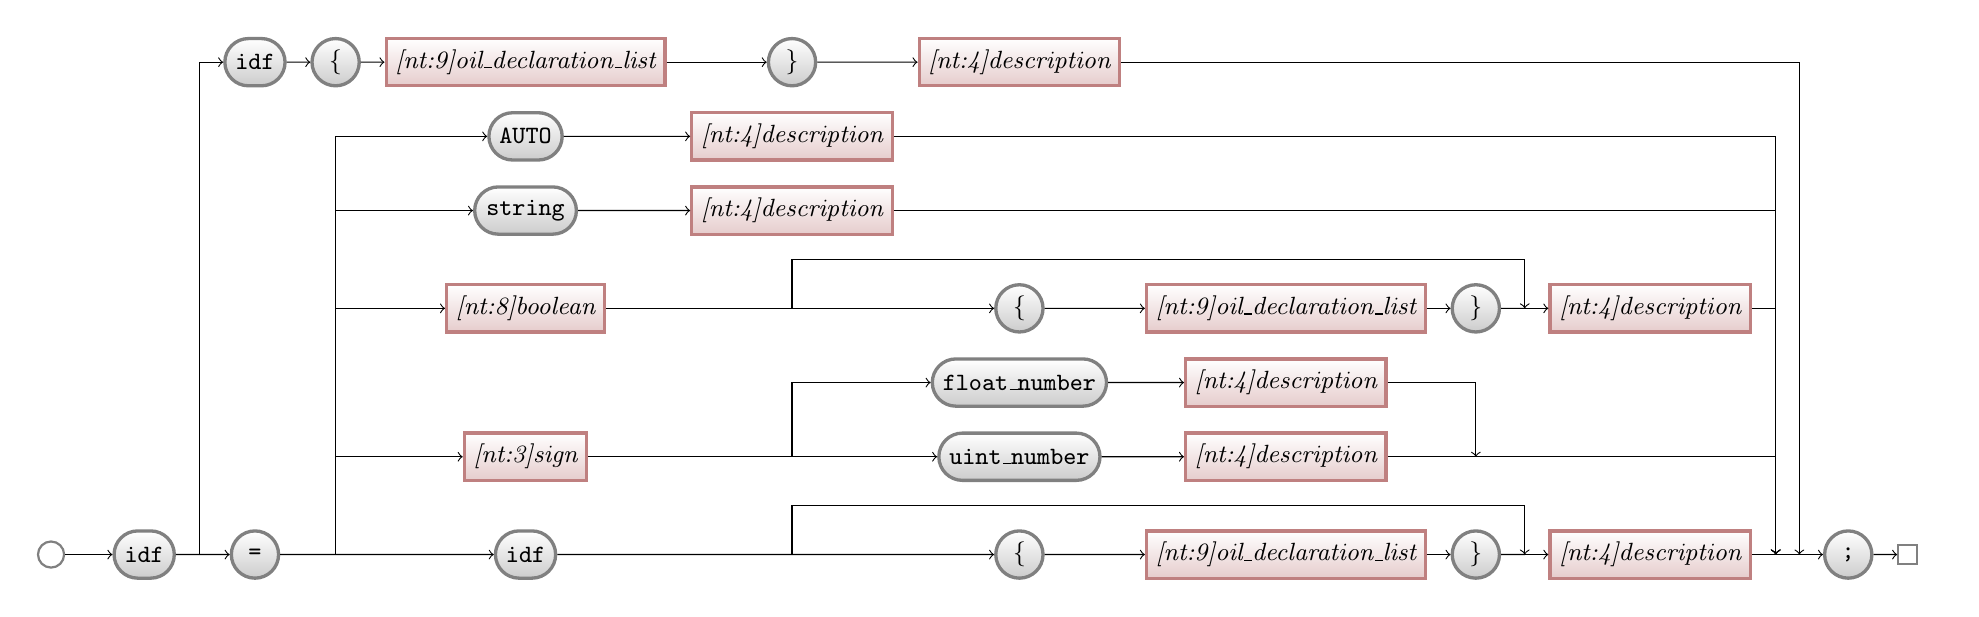
\begin{tikzpicture}
  \matrix[column sep=\ruleMatrixColumnSeparation, row sep=\ruleMatrixRowSeparation] {
    & & & & \node (p8-4) [terminal] {idf}; & \node (p8-5) [terminal] {\{}; & \node (p8-6) [nonterminal] {\nonTerminalSymbol{oil\_declaration\_list}{9}}; & \node (p8-7) [terminal] {\}}; & \node (p8-8) [nonterminal] {\nonTerminalSymbol{description}{4}}; & \\
    & & & & & & \node (p7-6) [terminal] {AUTO}; & \node (p7-7) [nonterminal] {\nonTerminalSymbol{description}{4}}; & \\
    & & & & & & \node (p6-6) [terminal] {string}; & \node (p6-7) [nonterminal] {\nonTerminalSymbol{description}{4}}; & \\
    & & & & & & & & \node (p5-8) [point] {}; & \\
    & & & & & & \node (p4-6) [nonterminal] {\nonTerminalSymbol{boolean}{8}}; & \node (p4-7) [point] {}; & \node (p4-8) [terminal] {\{}; & \node (p4-9) [nonterminal] {\nonTerminalSymbol{oil\_declaration\_list}{9}}; & \node (p4-10) [terminal] {\}}; & \node (p4-11) [point] {}; & \node (p4-12) [nonterminal] {\nonTerminalSymbol{description}{4}}; & \\
    & & & & & & & & \node (p3-8) [terminal] {float\_number}; & \node (p3-9) [nonterminal] {\nonTerminalSymbol{description}{4}}; & \\
    & & & & & & \node (p2-6) [nonterminal] {\nonTerminalSymbol{sign}{3}}; & \node (p2-7) [point] {}; & \node (p2-8) [terminal] {uint\_number}; & \node (p2-9) [nonterminal] {\nonTerminalSymbol{description}{4}}; & \node (p2-10) [point] {}; & \\
    & & & & & & & & \node (p1-8) [point] {}; & \\
    \node (P0start) [firstPoint] {}; & & \node (p0-2) [terminal] {idf}; & \node (p0-3) [point] {}; & \node (p0-4) [terminal] {=}; & \node (p0-5) [point] {}; & \node (p0-6) [terminal] {idf}; & \node (p0-7) [point] {}; & \node (p0-8) [terminal] {\{}; & \node (p0-9) [nonterminal] {\nonTerminalSymbol{oil\_declaration\_list}{9}}; & \node (p0-10) [terminal] {\}}; & \node (p0-11) [point] {}; & \node (p0-12) [nonterminal] {\nonTerminalSymbol{description}{4}}; & \node (p0-13) [point] {}; & \node (p0-14) [point] {}; & \node (p0-15) [terminal] {;}; & \node (p0-16) [lastPoint] {}; & \\
  };
  \draw[->] (P0start) -- (p0-2) ;
  \draw[->] (p0-2) -- (p0-4) ;
  \draw[->] (p0-4) -- (p0-6) ;
  \draw[->] (p0-6) -- (p0-8) ;
  \draw[->] (p0-8) -- (p0-9) ;
  \draw[->] (p0-9) -- (p0-10) ;
  \draw (p0-7) |- (p1-8) ;
  \draw (p0-10) -- (p0-11) ;
  \draw[->] (p1-8) -| (p0-11) ;
  \draw[->] (p0-11) -- (p0-12) ;
  \draw[->] (p0-5) |- (p2-6) ;
  \draw[->] (p2-6) -- (p2-8) ;
  \draw[->] (p2-8) -- (p2-9) ;
  \draw[->] (p2-7) |- (p3-8) ;
  \draw[->] (p3-8) -- (p3-9) ;
  \draw (p2-9) -- (p2-10) ;
  \draw[->] (p3-9) -| (p2-10) ;
  \draw[->] (p0-5) |- (p4-6) ;
  \draw[->] (p4-6) -- (p4-8) ;
  \draw[->] (p4-8) -- (p4-9) ;
  \draw[->] (p4-9) -- (p4-10) ;
  \draw (p4-7) |- (p5-8) ;
  \draw (p4-10) -- (p4-11) ;
  \draw[->] (p5-8) -| (p4-11) ;
  \draw[->] (p4-11) -- (p4-12) ;
  \draw[->] (p0-5) |- (p6-6) ;
  \draw[->] (p6-6) -- (p6-7) ;
  \draw[->] (p0-5) |- (p7-6) ;
  \draw[->] (p7-6) -- (p7-7) ;
  \draw (p0-12) -- (p0-13) ;
  \draw[->] (p2-10) -| (p0-13) ;
  \draw[->] (p4-12) -| (p0-13) ;
  \draw[->] (p6-7) -| (p0-13) ;
  \draw[->] (p7-7) -| (p0-13) ;
  \draw[->] (p0-3) |- (p8-4) ;
  \draw[->] (p8-4) -- (p8-5) ;
  \draw[->] (p8-5) -- (p8-6) ;
  \draw[->] (p8-6) -- (p8-7) ;
  \draw[->] (p8-7) -- (p8-8) ;
  \draw (p0-13) -- (p0-14) ;
  \draw[->] (p8-8) -| (p0-14) ;
  \draw[->] (p0-14) -- (p0-15) ;
  \draw[->] (p0-15) -- (p0-16) ;
\end{tikzpicture}

\nonTerminalSection{oil\_declaration\_list}{9}

\ruleSubsection{goil\_syntax}{goil\_syntax}{244}

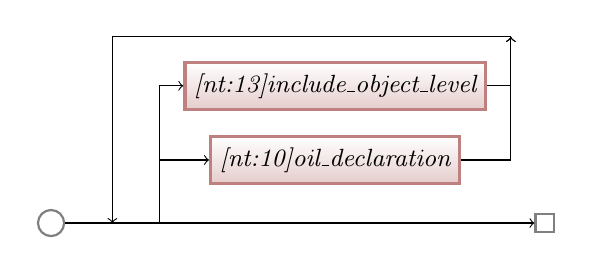
\begin{tikzpicture}
  \matrix[column sep=\ruleMatrixColumnSeparation, row sep=\ruleMatrixRowSeparation] {
    & & & & & & \node (p3-6) [point] {}; & \\
    & & & & & \node (p2-5) [nonterminal] {\nonTerminalSymbol{include\_object\_level}{13}}; & \\
    & & & & & \node (p1-5) [nonterminal] {\nonTerminalSymbol{oil\_declaration}{10}}; & \\
    \node (P0start) [firstPoint] {}; & & \node (p0-2) [point] {}; & \node (p0-3) [point] {}; & \node (p0-4) [point] {}; & & & \node (p0-7) [lastPoint] {}; & \\
  };
  \draw (P0start) -- (p0-3) ;
  \draw[->] (p0-4) |- (p1-5) ;
  \draw[->] (p0-4) |- (p2-5) ;
  \draw[->] (p3-6) -| (p0-2) ;
  \draw[->] (p1-5) -| (p3-6) ;
  \draw[->] (p2-5) -| (p3-6) ;
  \draw[->] (p0-3) -- (p0-7) ;
\end{tikzpicture}

\nonTerminalSection{sign}{3}

\ruleSubsection{goil\_syntax}{goil\_syntax}{126}

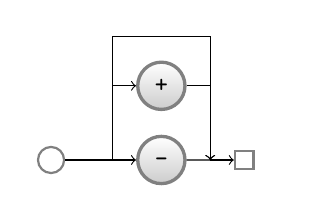
\begin{tikzpicture}
  \matrix[column sep=\ruleMatrixColumnSeparation, row sep=\ruleMatrixRowSeparation] {
    & & & \node (p2-3) [point] {}; & \\
    & & & \node (p1-3) [terminal] {+}; & \\
    \node (P0start) [firstPoint] {}; & & \node (p0-2) [point] {}; & \node (p0-3) [terminal] {-}; & \node (p0-4) [point] {}; & \node (p0-5) [lastPoint] {}; & \\
  };
  \draw[->] (P0start) -- (p0-3) ;
  \draw[->] (p0-2) |- (p1-3) ;
  \draw (p0-2) |- (p2-3) ;
  \draw (p0-3) -- (p0-4) ;
  \draw[->] (p1-3) -| (p0-4) ;
  \draw[->] (p2-3) -| (p0-4) ;
  \draw[->] (p0-4) -- (p0-5) ;
\end{tikzpicture}

\nonTerminalSection{start}{1}

\ruleSubsection{goil\_syntax}{goil\_syntax}{38}

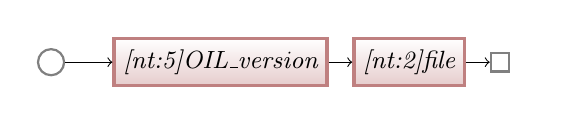
\begin{tikzpicture}
  \matrix[column sep=\ruleMatrixColumnSeparation, row sep=\ruleMatrixRowSeparation] {
    \node (P0start) [firstPoint] {}; & & \node (p0-2) [nonterminal] {\nonTerminalSymbol{OIL\_version}{5}}; & \node (p0-3) [nonterminal] {\nonTerminalSymbol{file}{2}}; & \node (p0-4) [lastPoint] {}; & \\
  };
  \draw[->] (P0start) -- (p0-2) ;
  \draw[->] (p0-2) -- (p0-3) ;
  \draw[->] (p0-3) -- (p0-4) ;
\end{tikzpicture}



\end{document}
